\documentclass[a4paper, 12pt]{report}




% Some highly suggested packages, please read their manuals.
\usepackage{cleveref}

\usepackage{natbib}

\bibliographystyle{apalike}

\usepackage[utf8]{inputenc}
\usepackage{color}
\usepackage[top=2.5cm, bottom=1.5cm, left=2.5cm, right=1cm]{geometry}
\usepackage[pdftex]{graphicx}
\usepackage{tikz}

% Logos
\newcommand{\ulb}{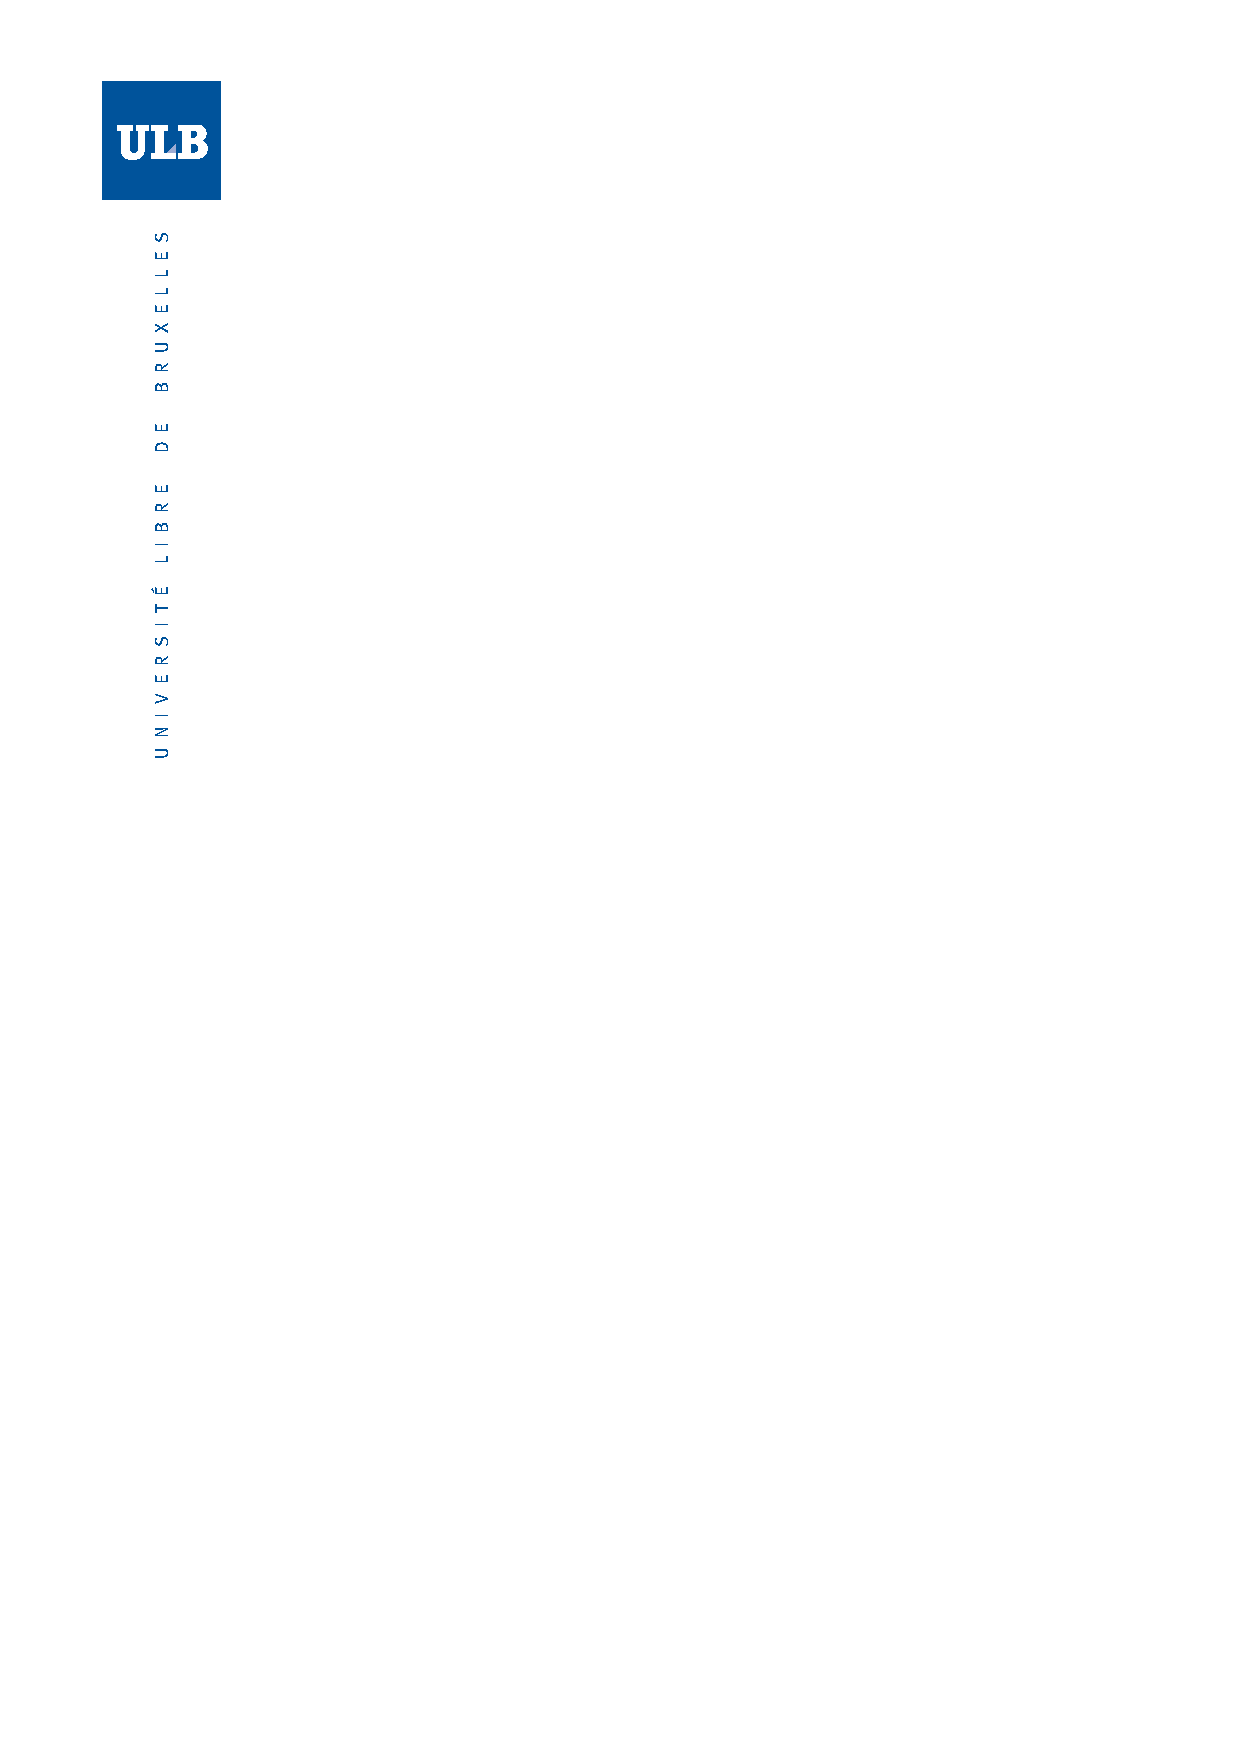
\includegraphics[scale=1.1]{logo_ULB2.pdf}}
\newcommand{\polytech}{
\includegraphics[scale=0.35]{logo_polytech_FR.pdf}}

% Polices
\definecolor{ULBblue}{rgb}{0,0.2196,0.5765}
\newcommand{\fontTitle}{\sffamily \Huge\selectfont \color{ULBblue}}
\newcommand{\fontSubtitle}{\sffamily \LARGE \selectfont \color{ULBblue}}
\newcommand{\fontText}{\sffamily \selectfont}
\newcommand{\fontColor}{\sffamily \selectfont \color{ULBblue}}

% Titre
\newcommand{\titleA}{\fontTitle{Première ligne de titre du mémoire}} % Titre identique au titre remis au secrétariat
\newcommand{\titleB}{\fontTitle{Deuxième ligne de titre du mémoire}} % (dans la langue de rédaction a priori)
% Sous-titre
\newcommand{\subtitle}{\fontSubtitle{Ligne du sous-titre du mémoire}}
% Titre du diplôme
\newcommand{\diplomaA}{\fontText{Mémoire présenté en vue de l’obtention du diplôme}} % A laisser en Français
\newcommand{\diplomaB}{\fontText{d'Ingénieur Civil [...] à finalité [...]}}

% Etudiant
\newcommand{\student}{\textbf{\sffamily \large [Prénom Nom]}}

% Supervision
\newcommand{\promAa}{\fontColor{ primary eur}}
\newcommand{\promAb}{\fontText{Professeur [Prénom Nom]}}
\newcommand{\promBa}{\fontColor{Co-Promoteur}}
\newcommand{\promBb}{\fontText{Professeur [Prénom Nom]}}
\newcommand{\promCa}{\fontColor{Superviseur}}
\newcommand{\promCb}{\fontText{[Prénom Nom]}}
\newcommand{\deptA}{\fontColor{Service}}
\newcommand{\deptB}{\fontText{[Nom du service]}}

% Année académique
\newcommand{\yearA}{\fontColor{Année académique}}
\newcommand{\yearB}{\fontText{20xx - 20xx}}

\begin{document}

	\thispagestyle{empty}
	\newgeometry{top=2.5cm, bottom=1.5cm, left=2.5cm, right=1cm}
	\setlength{\unitlength}{1mm}
	\noindent\begin{picture}(175,257)
	
		\put(0,245){\polytech}
		\put(153,139.5){\ulb}
		
		\put(8,155){\makebox(150,10)[l]{\titleA}}
		\put(8,145){\makebox(150,10)[l]{\titleB}}
		\put(8,135){\makebox(150,10)[l]{\subtitle}}
		
		\put(0,75){
		\begin{tikzpicture}[scale=0.1]
		\fill [fill=ULBblue](0,0) rectangle (0.8,90);
		\fill [fill=ULBblue](0,57) rectangle (152,57.8);
		\end{tikzpicture}}
		
		\put(8,120){\makebox(150,5)[l]{\diplomaA}}
		\put(8,115){\makebox(150,5)[l]{\diplomaB}}
		
		\put(8,75){\makebox(150,10)[l]{\selectfont \student}}
		
		\put(8,44){\makebox(80,5)[l]{\promAa}}
		\put(8,39){\makebox(80,5)[l]{\promAb}}
		\put(8,31){\makebox(80,5)[l]{\promBa}} % Commenter la ligne si pas nécessaire
		\put(8,26){\makebox(80,5)[l]{\promBb}} % Commenter la ligne si pas nécessaire
		\put(8,18){\makebox(80,5)[l]{\promCa}} % Commenter la ligne si pas nécessaire
		\put(8,13){\makebox(80,5)[l]{\promCb}} % Commenter la ligne si pas nécessaire
		\put(8,5){\makebox(80,5)[l]{\deptA}}
		\put(8,0){\makebox(80,5)[l]{\deptB}}
		
		\put(145,5){\makebox(30,5)[r]{\yearA}}
		\put(145,0){\makebox(30,5)[r]{\yearB}}
	
	\end{picture}
	\restoregeometry



\chapter{Introduction}
Social network analysis is an interdisciplinary discipline originally developed under the influence of sociology and mathematics \citep{history_social}. It consist of using graph and network theory to represent links among individuals as a network in order to analyze them. \\

Research in computer science are developing semantically-oriented techniques to analyze fiction. \cite{character_country} had presented a method to extract social network from literary which allows to apply Social Network Analysis techniques on it. \cite{movie} presented a method to extract a social network from movies. \\

This master thesis consists firstly in the development of a software that extracts social networks from novels and movie scripts. Secondly it consists in the analysis of the topology of the extracted networks. The software has been originally developed during an other master thesis \citep{original} and was only working on novels. For this reason I will focus on the modification that I have made and the evolution of the state of the art since this period. 


\chapter{Extraction of the network}
\section{Character identification}
``Character identification consists in detecting which characters appear in the considered narrative, and when exactly they appear in this narrative'' \citep{fiction}. The first step is very easy with scripts as the characters speaking in each dialog are manually annotated.
However novels don't contain such annotations and the set of characters has to be extracted from the text. A method has been developed to respond to this problem. In both cases, the second step is easier and consists only in binding each occurrence of character mention to the corresponding character.

\subsection{Character extraction in Novels}
According to \cite{fiction},  character in novels may appear on the form of a proper noun, a pronoun or an anaphoric noun phrase. Proper nouns that are composed of a single word are called proper names. In this work, character are only detected when they are on the form of a proper noun. This choice is motivated by the fact that characters will be later connected when they are mentioned in the same conversation. The cost of this simplification is the lost of smaller characters that appears only under the form of an anaphora. I considered that in most cases, a character taking part in a conversation is mentioned at least once under the form of a proper noun. In our situation, the first step of \textit{character identification} on a written support is the extraction of names that represents the characters and the linking of aliases (names that refers to the same character). Once all extracted names are bound with a character, each occurrence of a name in the story signal the appearance of the associated character. As the task of extracting a set of proper nouns and binding aliases is error-prone, some authors decided to do it manually \citep{agarwal-etal-2013-automatic}.  \cite{he-etal-2013-identification} proposes to build automatically a list of character from wikipedia but this method has the disadvantage to focus only on main characters and to be dependent on external information unavailable for some stories.  Here we will focus on automatic method because they can be used on many different text with a minimal pre-processing.\\

A major modification of the program concern this first step of the character identification process. The original process was only considering that a character could be represented by a proper name and was linking names that appears together more than 1 times over 3. But using only proper names over all proper nouns is a simplification that makes the program loose a lot of information. The use of proper nouns makes the binding of nouns more complex but the current state of the art contains method to perform this task. \\
 
 \begin{tabular}{lll}
\textbf{chunk} & \textbf{names extracted using proper nouns} &  \textbf{names extracted using proper names} \\
   Ron and Hermionne & Ron AND Hermionne & Ron\\
   you Mr. H. Potter & Mr. H. Potter &  Potter\\
   dear Harry Potter & Harry Potter & Harry OR Potter \\
   James Potter& James Potter & James OR Potter \\
   yer brother Charlie & Charlie & Charlie\\
\end{tabular}

\subsubsection{Name Entity Recognition}
The task of labeling group of words as Entity is called Name Entity Recognition (NER). Those entity includes \textit{person}, \textit{location} and \textit{organisation} \citep{libraries}. This is the most common way to extract characters names from a novel.
The best NER methods are supervised or semi-supervised and trained with annotated datasets of news, text from social media or biomedical data \citep{NER_survey_recent}. This decreases their performance on novels, especially novels from fantasy or the older ones \citep{NER}.  Unsupervised methods typically rely on rules and domain-based knowledge, it makes them completely domain dependent. POS-tagger may be considered as naive program of NER. The original software \citep{original} was extracting all words labeled as proper names by a POS-tagger with the major issue of considering only single-word names while in \cite{quoted}, proper names are tagged using a POS-tagger and contiguous proper names are considered as a proper noun. \cite{character_meta} also extracts subjects of verbs present in a dataset of verbs strongly associated with ``person'' entity. This techniques allows to detect anaphoric nouns and not only proper nouns. \\
Pattern the NLP  library of python that is used in the software doesn't have any NER module. Spacy, another NLP-library of python have an available module that performs NER using `Conditionnal Random Fields', a statistical model that uses supervised learning. Pre-trained model are available but the model could also be trained manually with an annotated dataset.

\subsubsection{Unification of Character Occurrences}
Unification of Character Occurrences is the task of unifying all mentions of a same character in a narrative \citep{fiction}. When only proper nouns are considered, this task can be simplified into Alias Resolution: the linking of all names that refers to a same characters and the making a differentiation between names that refers to different characters \citep{book_social}.\\
The binding of names can be done using a measure of string similarity, set of rules or using meta-information of strings such as an inferred gender. In multi-stage methods, proper nouns are are divided between cluster, each of them being associated to a single character. The clusters are merged following a sequence of conditions. Multiple methods have been developed to solve this task with their own specificity without that one method stand out from others.\\
The original software \citep{original} was linking proper names that appears together 1/3 of the times to link first name with last name with the major inconvenience of binding different characters sharing a same first name or last name and leaving unbound name and lastname of characters that are more frequently called by only one of those words. 
However most of the state of the art methods focuss on proper nouns: \cite{delete5} discards all proper nouns that appears less than 5 times, then try to bind multi-words nouns between them before binding them with single words nouns. \cite{structure_clustering} also classify names into multiple classes and apply different rules on those classes. \cite{character_meta} propose to bind nouns that share words except in some cases, such as nouns sharing a last name but having a different first name. \cite{variation} proposed a method to bind entity representing art object by generating variations of proper nouns and linking them with names corresponding to those variations, this method have been applied on characters detection in novels by \cite{quoted, character_meta}.  In \cite{delete5, structure_clustering, quoted},  a gender is inferred from each proper nouns using a list of masculine and feminine first names and gendered titles to avoid to merge cluster of names having different genders. It ends by removing infrequent characters, characters whose the total number of apparition of the cluster of names  is smaller that a threshold. This should reduce the number of ``false positive'' characters (cluster of names that are not related with a character), at the cost of minor character. \cite{delete5} draws the conclusion that all methods are error-prone and that the difficulty to obtain annotated data on this task makes any comparison between the different methods very difficult. Even with a dataset containing all characters present in a narrative, the presence of multiple aliases would makes the evaluation of the character extraction very difficult.  \\

Some methods also use co-reference resolution tools to link characters mentions between each others \citep{character_meta}. Coreference resolution tools are program that automatically clusters mention in text that refers to the same entity. They do it using neural networks and are especially used to link names with pronouns or anaphoric noun phrase \citep{coref_deep, coref_deep2} . This is useless to the software here as those form of references are not used in this work. \\

\subsection{Proposed method of character extraction in novels}
As explained in the previous section, the method here extract proper nouns, the extracted nouns are composed of multiple words including honorifics. Also only proper nouns are extracted, anaphoric noun phrase are ignored. The method consist of a multi-pass algorithm that passes 2 times over chunks to extract a list of nouns,  classify them and then pass 5 times over the set of nouns to bind aliases.
\subsubsection{Names Entity Recognition}
A Name Entity Recognition method has been designed to extract characters names from novels. This technique uses a POS-Tagger to extract proper names from the text and several collection of proper names commonly used in English to isolate characters names. Then proper nouns are extracted from chunks containing proper names. The collection of words contain a list of countries, nationalities, honorifics (classified following the related gender), stop-words, profanities, words related to time and words related to the academic domain. In this method, a  proper name is considered as \textit{valid} if it begins with a capital letter but is not composed with capital letters only. The assumption has been made that proper names contains more than one letter.\\
First of all the POS-tagger is passed on the head word of all chunks to extract  proper names. The POS-tagger used is the one developed by the python library pattern which classify  proper names whether they are related to a location or not. If a word is not labeled as a location, the algorithm considers the word as a proper name if it doesn't appear in the lists of English  proper names and is not the first word of a sentence. First words of sentences are not kept as they are capitalized and so they are more likely to be wrongly classified as proper names. The assumption is made that proper names will appear several time and that at least one of those appearance will not be at the begin of a sentence. Proper names and  proper names related to locations are saved with the number of their appearance.\\
Secondly the algorithm check that words labeled as location don't appear in the list of proper names. In such cases, the word will be removed from the list of proper names if it appeared more often as a location than as a name.\\
The final step of the Names Entity Recognition method consists of extracting proper nouns from proper names. All chunks containing a proper name are isolated.   Then all sequence of consecutive valid  proper names are extracted and considered as proper nouns. For instance from the chunk ``Mr Harry Potter and Ron'' 2 proper names are extracted: ``Mr Harry Potter'' and ``Ron''. The proper nouns are registered with the number of their appearance.\\

\subsubsection{Proper nouns classification}
All the extracted proper nouns are classified following their gender and their form to make easier the alias resolution. The classification of genders is also used to produce gender-related information about the topology of the network.\\
Firstly all the names are parsed using the python tool \textit{HumanName} from the library {NameParser}. It separates words contained in a noun in a list of honorifics, first name and last name.\\

To infer the gender, the algorithm will used the list of honorifics classified by gender and a list of gender related first name. The gender of nouns containing a first name from the list of first name or an honorific from the list of  labeled honorifics will be assigned. If multiple words in the noun are related to different genders, the majority vote is used. After this phase all nouns are labeled as \textit{masculine}, \textit{feminine} or {neutral}.

Then a category will be assigned to each words following their forms:
\begin{enumerate}
	\item The first category contains nouns that have at least an honorific, a first name and a last name.
	\item The second one contains nouns with a first name and a last name but no honorific.
	\item The third category contains nouns with an honorific and a first name but no last name.
	\item This category contains nouns with an honorific and a last name but no first name.
	\item The fifth category contains the remaining nouns.
	 \item If the first name of a noun is not in the list of proper noun and doesn't respect the criteria to be labeled as proper noun, the noun is considered as an error and is removed.
\end{enumerate}

\subsubsection{Alias resolution}
The alias resolution process consist of a multi-pass algorithm that firstly creates  primary link and secondary link between all  nouns, then  transforms secondary link into  primary link in some cases. After this linking phase, cluster are  build to represent character. Each cluster consists of nouns connected between them by a path of primary link. The most used noun of the cluster is called the head of the cluster and is used to represent the associated character in the social network. In the following explanations, I will speak about ``compatible genders'' between 2 nouns, it means that the gender assigned to those nouns doesn't prevent them to point the same character. Concretely they have the same gender or one of them is neutral. To be connected, nouns have to have compatible genders. Once two nouns are linked by a  primary link, if one of them was gender neutral, its gender will be inferred from its neighbor. In such situations the neutral word will delete all its connections with words of the opposite gender. In the following explanation I will also speack about "primary-connection" or secondary"neighbors"to speak about names connected using a path of primary link and names neighbors from each other by a secondary link. \\

During the first pass, all first name used by nouns of class <3  are taken one by one. Diminutive and nicknames associated to a first name are looked in the set of proper names. Then all proper nouns that possess that first name, a diminutive or a nickname are grouped. In some cases the first name, the diminutive or the nickname has been labeled as last name in other nouns, those nouns are also added. For each pair of nouns from this group that have compatible genders, the nouns are linked
\begin{itemize}
\item
	 using a  primary link if:
	\begin{itemize}
	\item they have the same last name and their first name is the original first name, a diminutive or a related nickname. This also works with nouns that don't have last name as they last name is considered to be the empty string.  For instance: ``D Dursley'' and ``Dudley Dursley''. 
	\item if both of the names have an empty last name or first name. In this case the algorithm consider that they share a same first name/last name even if it is possibly labeled differently in each noun. For instance:``Mr Flitwick'' and ``Professor Flitwick''.
	\end{itemize}
	Once 2 nouns are connected with a  primary link, if one of them was neutral, he will receive the gender of the other word.
\item
	 using an  in primary link if:
	\item  their first name is the original first name, a diminutive or a related nickname and only one of them have an empty last name. 
	\item if one of them have an empty first name.
	Secondary  link represent a potential connection between names which could be unrelated. For instance ''Mr Durlsey'' could be related to ``Dudley Dursley'' or to ``Vernon Dursley'', so he will be linked using a secondary link to both of them. ``Harry Potter'' and ``James Potter'' should not be linked as it appear clearly that this is 2 different character sharing a last name.
\end{itemize}

In a second phase, all last name are taken one by one. Last name that has also been used in previous pass as a first name are not considered because they are likely to be incorrectly labeled. All nouns sharing the last name or a diminutive are grouped. For each pair in this group, if they have compatible genders, they are linked using:
\begin{itemize}
\item a  primary link if both of their firstname are empty. 
\item an in primary link in other cases.
\end{itemize}

Once these phase have been completed, we will observe secondary link and separate those who are due to a true connection between 2 names and the links that should be removed.  We will takes the nouns that contains the less information and try to link them with the nouns that are more likely to be their neighbors. The chosen neighbors is the most common noun among the neighbors. This technique will result in some errors but their numbers should be limited.
\\
The third pass focuses on neutral nouns of category 1 and 2. We will try to find them a gendered alias among their potential partners. Firstly each of them will be grouped with all nouns connected to him using  primary links. Then a second group will be formed with all they secondary-neighbors. Iteratively the most common neighbors  will be removed from the second group and linked to the first group using a  primary  connection. If the noun is gendered, the gender will be assigned to all word from the first group and the process will end. If the noun is also neutral, all nouns  primary ly connected to it will be added to the first group and again the most common noun from the second group will be chosen to be linked with the first group. 
\\
The fourth and fifth pass focus on words from the 3-4-5 categories that are not connected with nouns from the 1-2 categories. Those words consists of a single first name or last name and should be linked to the most common character having this name. Again in the forth pass they are grouped with the primary-connected nouns. The most common noun among their secondary neighbors of 1-2 categories is added to the group and  primary ly linked with it. But nouns that are not linked to any 1-2 nouns will remain unbound. In the fifth pass, all secondary links between those names will be iteratively transformed into primary link. Link between nouns that becomes incompatible due to their gender during the process, are removed.
\\
In the last part of the algorithm, cluster are made with words primary-connected and the most common noun of each cluster is chosen as  head of the cluster.
\\

\subsubsection{Detection of potential speaker and listener}
All the sentence of the text are separated in 2 categories: the sentence that are part of dialogues and sentences that are part of context description between dialogues.
In dialogues, the object and subject of each sentence are designated as potential listener and speaker. In contexts, only the subject is extracted as potential speaker of the context which will be further used to detect speakers of the following dialog. \\
The extraction is made using the pattern POS-tagger. Initially the entity extracted were chunks but the program has been modified to look for proper nouns.\\

\subsubsection{Extraction of character}
\textbf{Original paper}:
The extraction of characters is made using a 2 pass algorithm.
\begin{enumerate}
    \item \textit{First pass}: Reading of all headwords of chunks to detect proper nouns. For each chunk of each dialog context, if the main word is labelled as a proper noun, is composed of at least 3 letters and is not only uppercase. Proper nouns are added to the list of proper names, their number of appearance is recorded and the associated chunks are stored.\\
    \item \textit{Second pass}: Reading of all chunks to check if some proper names appear in the same chunk.
    \item Pairing of proper names if the less common appear with the most common more than 1 times over 3.
    \item Pairing of proper nouns sharing a common root.
    \item Paired nouns are clustered and considered as aliases. The name that appear the most in each cluster will be used to represent all the cluster in the social network. The chunks stored by other names of the cluster are now linked with the most appearing name. They will be use to identify the character from a potential speaker.
\end{enumerate}{}

\textbf{Problem encountered by the algorithm}
Firstly the first pass detecting proper nouns causes many false positive. Some words are labeled as NP by the tagger without being capitalize, some words are capitalized and incorrectly labelled as NP because they are the first word of a sentence or refer to a  proper name which is not a name. A non proper name incorrectly labelled a single time over multiple appearance will be considered as a proper name.\\
Example of words incorrectly labeled as proper names :\\
'gruffly', 'Saturday','Transfiguration',"You'd","Uncle","Yeah", "Wizard", "London". 
Te high number of false positive increase a lot the number of characters and make the structure of the network non trustful.
On the book "Harry Potter 1" detected characters have been manually labelled as true positive or false positive. Only 69 over 193 are labeled as true positive.\\

The fact that proper nouns are only composed of a single token makes the identification of characters in multiple way. \\
The pairing is needed to link firstnames and lastnames of characters but in some cases multiple proper nouns that should not be linked appear in the same chunk.\\  
Here are some common mistakes in character extraction with example from the book "Harry Potter 1".
\begin{enumerate}
    \item \textbf{When both the firstname and the lastname of a character are used to identify him, they are not paired}: "Harry" and "Potter" are labelled as different character.
    
    \item \textbf{When multiple characters share the same firstname or lastname, if the linking is made they will all be clustered as a single character}: the names refering the 8 characters of the "Weasley" family are mixed in 4 cluster. Each cluster is composed of aliases refering to 2, 3 or 4 characters.
    
    \item \textbf{Some characters are refered with proper nouns that should not be used for pairing}: "Mr" is paired with "Dursley" and "Weasley" because the text often refer to "Mr Dursley" or "Mr Weasley". It causes the clustering of unrelated words. The same problem appear with other title like "professor". 
    
    \item \textbf{Some chunks contain multiple characters}: The algorithm link to a single character the chunks "Ron and Hermionne", "Mr and Mrs Weasley" or "Fred and George".
    
\end{enumerate}


\textbf{New algorithm}: The new algorithm use also 2 pass and is based on multiple-tokens names. It uses the first pass on the previous algorithm with additional conditions to detect proper nouns and then extract the multiple-tokens proper names during a second pass.


\begin{enumerate}
    \item \textit{First pass}: All chunks are read and the proper names are extracted from the chunk headword. To diminish the number of false positive, they should answer to multiple conditions to be extracted:
    \begin{itemize}
        \item The POS-tagger label it as NNP but not as a location (tag NNP-Loc).
        \item The word is capitalized but not entirely uppercase.
        \item The word is not the first word of a sentence.
        \item The word doesn't belong to a set of words that has been registered as non proper names. This set of words is the union of a set of english honorifics and a set of common english word provided by the library pattern.
    \end{itemize}
    \item \textit{Second pass}: multi-tokens proper names are extracted from all the chunks headed by a proper noun. The number of appearance of each proper names is stored.
    
    \item All proper names are analysed and split between a firstname, a lastname and an honorific. Their gender is infer from the lastname and the honorific when it is doable. They are classified following the composant that the name has. If a firstname has not been considered as a proper name but answer to the conditions, it is added to the list of proper names.
    
    \item Names sharing the same firstname or lastname are linked together. 2 firstnames that appear together in a list of english nicknames or sharing a common root are considered as the same firstname. 2 type of linking are produced:\\ 
    The 1-linking that pairs immediately names having a lot in common. If one of the names gender was labelled as neutral, its gender is infer from the gender of the second name. \\ 
    The 2-linking makes 2 names potential pair. If the assigned gender of the names were not the same, its not modified.\\
    2 names labeled as male and female can not be paired.
    
    \item Group of paired genderless names are paired with their gendered 2-value neighbor having the bigger number of appearance. Their gender is inferred from the gender of this neighbor.
    
    \item Group of paired names without firstnames are paired with their most common neighbor having a firstname. 
    
    \item All the aliases are divided in cluster. A cluster is formed by a group of names such that it exist a 1-value path that link all of them. Each cluster designates a character. The most common name of each cluster is chosen as the headname and will be used in the network to designates the character. 
    A new  primary ed graph is build where each alias is pointing his headword. 
    %37/109
\end{enumerate}

%\textit{Proper names detection}: For each chunk of each dialog context, if the main word is labelled as a proper noun, is composed of at least 3 letters and is not only uppercase, this noun is added in the alias table.\\
%\textit{Aliases detection}: All chunks are read again and the program compute the number of times that each pair of proper names appear together in a chunk. If 2 words appear more than 2/3 of the time together, they are considered as alias.


\textbf{Actor identification}:\\
For each sentence of a conversation(dialog + context), the algorithm try to extract potential speakers and potential listeners.
The subjects of the context are considered as potential speakers. Any proper names appearing in the context and being the subject of an other sentence are also taken. The subjects and objects extracted from the dialog are considered as potential listeners.
\\
\textbf{Alias coresolution}:\\
Then an alias-table is constructed:\\
First pass: For each chunk of each dialog context, if the main word is labelled as a proper noun, is composed of at least 3 letters and is not only uppercase, this noun is added in the alias table.\\
Second pass: If 2 words from the alias table appear more than 2/3 of the time together, they are considered as alias.



Modification:
To be considered as a potential character, nouns have to be:
\begin{itemize}
    \item Be labelled as proper noun but not as an location.
    \item Begin with a capital letter.
\end{itemize}


\bibliography{biblio} 
%\printbibliography%

\end{document}

% Template conçu par Benjamin Vanhemelryck et revu par François Bronchart - Mai 2013